\documentclass[10pt,a4paper]{article}
\usepackage[utf8]{inputenc}
\usepackage[czech]{babel}
\usepackage[T1]{fontenc}
\usepackage{graphicx}\usepackage{lmodern}
\usepackage[top = 2cm, bottom = 2cm, left = 2cm, right = 2cm]{geometry}
\usepackage{fkssugar}
\usepackage{url}
\usepackage{tocloft}
\usepackage{ulem}
\usepackage{subcaption}
\addto\captionsczech{\renewcommand{\refname}{\tiny}}

%For title page
\usepackage{titlesec}
\usepackage{setspace} %Rámeček nahoře
\usepackage{framed} %Rámeček nahoře
\usepackage{array} %Tabulka dole
%for graph
\newcommand{\listgraphname}{\LARGE SEZNAM GRAFŮ}
\newlistof{graph}{exp}{\listgraphname}
\newcommand{\graph}[1]{%
\refstepcounter{graph}
\par\noindent\small{Graf \thegraph: #1\\[0.5cm]}
\addcontentsline{exp}{graph}
{\hspace{0.7cm}\protect\numberline{\thegraph}\hspace{0.3cm}#1}\par}


\begin{document}


\thispagestyle{empty}
\newgeometry{top = 2.5cm, bottom = 0cm, left = 2.5cm, right = 3cm}

{%T tomto je uzavřena celá titulka
%Tloušťka rámečku
\setlength{\fboxrule}{1.5pt}

\noindent
\framebox{
\begin{minipage}{\textwidth}
\setlength{\parindent}{17.62482 pt}
\phantom{d}

\begin{minipage}{0.6\textwidth}
{
\Large Kabinet výuky obecné fyziky, UK MFF\\
}
\vspace*{0.2cm}

{
\bfseries
\huge Fyzikální praktikum IV%ČÍSLO
}
\end{minipage}
\begin{minipage}{0.4\textwidth}
\begin{center}
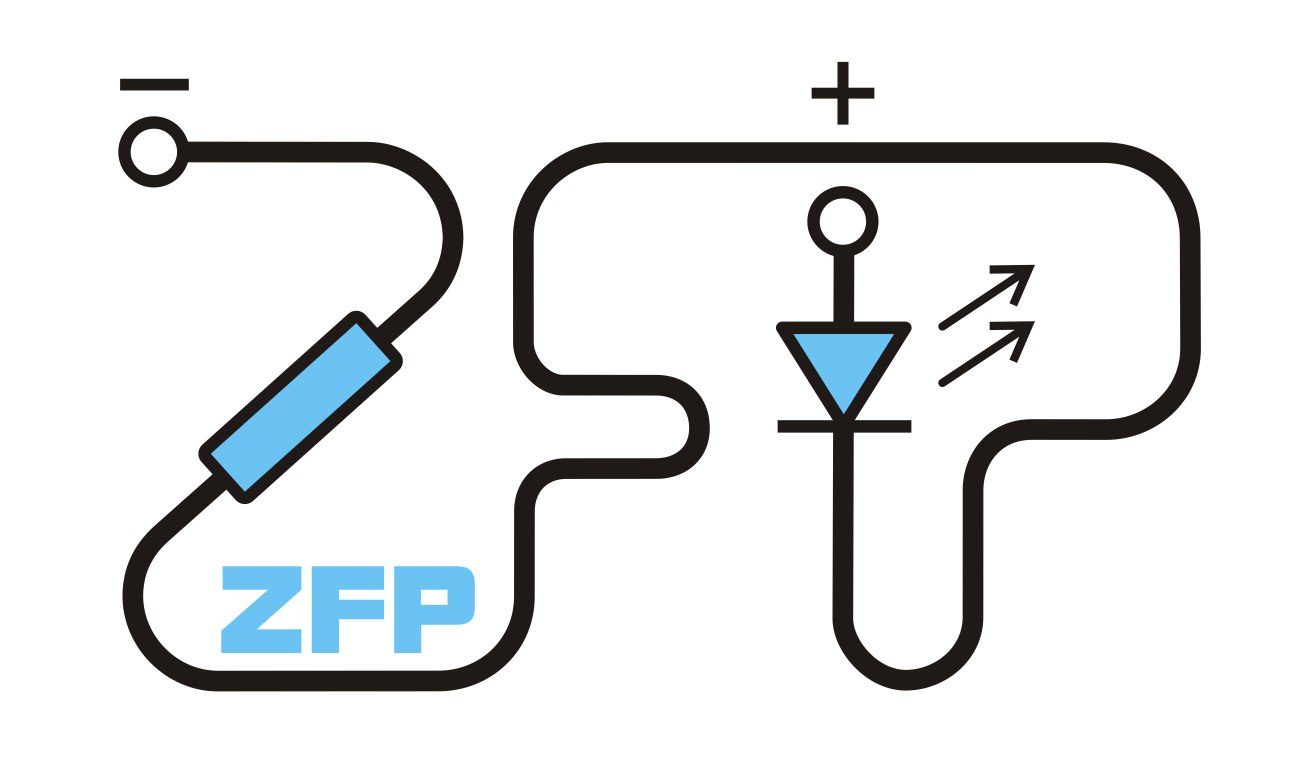
\includegraphics[width=4.5cm]{ZFP.jpg}
\end{center}
\end{minipage}\\\\

%\vspace*{0.5cm}

{
\setstretch{1.5}
\Large
\noindent
Úloha č. A7 %Číslo

\noindent
Název úlohy: Pozitronová emisní tomografie%Název

\noindent
Jméno: Kateřina Rosická%Jméno

\noindent
Datum měření: 5. října 2021%Datum TODO

\phantom{d}
}
\end{minipage}
}
%Konec horního rámečku

{
\phantom{d}

\Large
Připomínky opravujícího:\\
\vspace*{6.75cm}
}

\newcommand{\linka}{\noalign{\hrule height 1pt}}
\newcommand{\linkadva}{\noalign{\hrule height 1.5pt}}
\setlength\extrarowheight{9.5pt}
\Large
\noindent
\begin{tabular}{!{\vrule width 1.5pt} l !{\vrule width 1pt} c !{\vrule width 1pt} c !{\vrule width 1.5pt}}
\linkadva
& Možný počet bodů & Udělený počet bodů \\\linkadva
Teoretická část & 0--2 & \\\linka
Výsledky a zpracování měření & 0--9 & \\\linka
Diskuse výsledků & 0--4 & \\\linka
Závěr & 0--1 & \\\linka
Použitá literatura & 0--1 & \\\linkadva
\hspace*{\fill} \textbf{Celkem} \hspace*{\fill}& max. 17 & \\
\linkadva
\end{tabular}
\phantom{d}

Posuzoval: \hspace*{\fill}dne:~~~~~~~~~~~~~~~~~

}%Konec uzavření titulky
\newpage
\newgeometry{top = 2cm, bottom = 2cm, left = 2cm, right = 2cm}
\setcounter{page}{1}


%-------------------- ZAČÁTEK PROTOKOLU ------------------------

\section*{Pracovní úkol}
\begin{enumerate}
\item[] {\it Měření s jedním zářičem}
\item Poté, co vyučující umístí silnější zářič $^{22}$Na do stojánku, změřte úhlové rozdělení koincidencí v oblasti úhlů potřebné pro nalezení polohy zářiče, doba měření $"20 s"$. Vysvětlete tvar naměřeného úhlového rozdělení, získané poznatky využijte při domácím zpracování.
\item Změřte četnost koincidencí pro úhly $\Phi = "60\dg", "90\dg", "120\dg"$ bez plechu a $"120\dg"$ s Pb plechem mezi detektory, doba měření $"100 s"$. Vysvětlete pozorované četnosti.
\item[] {\it Měření se dvěma zářiči}
\item Poté, co vyučující přidá do krabičky druhý zářič, změřte úhlové rozdělení koincidencí s krokem $"5\dg"$.
\item Zvolte aspoň 2 další vhodné úhly otočení krabičky $\Psi$ a opakujte měření 3).
\item Narýsujte přímky spojující detektory do obrázku připraveného u úlohy a odečtěte polohu průsečíku - polohu zářiče vůči krabičce. Pozn.: Při volbě otočení krabičky $\Psi$ se můžete řídit polohou už zakreslených průsečíků.
\item Vzdálenost detektoru od zářiče zakresleného na obrázku porovnejte s měřením skutečné vzdálenosti.
\item[]{\it Při domácím zpracování dat}
\item Polohy zářičů vůči krabičce určujte pomocí vztahů a metod popsaných v návodu. Podle výsledků zpracování nakreslete obrázky analogické k obrázkům narýsovaným během praktika. Chyby polohy zářičů určete graficky.
\end{enumerate}
\section*{Teorie}
\subsection*{Anihilace pozitronu}
Pozitronová emisní tomografie je zobrazovací technika využívající se v lékařství. Je založena na zavedení radiofarmaka - beta plus zářiče - do tkáně, kde emituje pozitron, který ve tkáni uletí několik desetin milimetru, než anihiluje s elektronem. Ze zákona zachování energie pak mají vznikající kvanta gamma záření energii rovnou součtu klidových energií elektronu a pozitronu a ze zákona zachování hybnosti pak mají opačně orientované hybnosti a shodnou energii $"511 MeV"$.
\subsection*{Koincidenční měření}
Měření jsme prováděli takzvaným koincidenčním měřením, které detekuje impulz pouze tehdy, když na obou detektorech jsou detekovány impulzy s časovým rozdílem menším než nastavený interval, který pro naše měření byl přibližně $\tau="0,8 \micro s"$
Anihilační měření zde využíváme právě proto, abychom na detektoru rozlišili fotony pocházající ze stejného rozpadu, využijeme právě koincidenční měření. To však může kromě skutečného signálu detekovat i náhodné koincidence, a to s četností $N_a=2N_1N_2\tau$, kde $N_1$ a $N_2$ jsou četnosti signálů na jednotlivých detektorech.
\subsection*{Experimentální uspořádání}
V experimentu používáme lebku se zářiči obklopenou dvěma detektory A a B, s tím, že detektor A je pevně umístěn na podložku, krabička otáčíme o úhel $\Psi$ a detektor B otáčíme o úhel $\Phi$. Uspořádání můžeme vidět na obrázku \ref{usporadani}.
\begin{figure}[h]
\centering
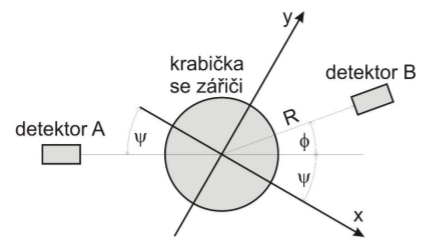
\includegraphics{usporadani.png}
\caption{Experimentální uspořádání, převzato z \cite{studijnitext}}
\label{usporadani}
\end{figure}
Pro polohy detektorů pak v soustavě souřadnic spojených s lebkou platí:
\eq{\begin{array}{cc}
x_A=-R\cos{\Psi}&x_B=R\cos{(\Psi+\Phi)}\\
y_A=-R\sin{\Psi}&y_B=R\sin{(\Psi+\Phi)}
\end{array}
}
Nejistoty těchto poloh určíme metodou přenosu chyb pomocí nejistoty měření vzdálenosti $\sigma(R)$ a nejistot úhlů $\sigma(\Psi)$ a $\sigma(\Phi)$:
\eq[m]{
\sigma(X)&=\sqrt{\(\pder{X}{R}\sigma(R)\)^2+\(\pder{X}{\Psi}\sigma(\Psi)\)^2+\(\pder{X}{\Phi}\sigma(\Phi)\)^2}\\ \label{prenoschyb}
\sigma(x_A)&=\sqrt{(-\cos{\Psi}\sigma(R))^2+(R\sin{\Psi}\sigma(\Psi))^2}\\
\sigma(x_B)&=\sqrt{(-\cos{\Psi}\sigma(R))^2+(R\sin{\Psi+\Phi}\sigma(\Psi))^2+(R\sin{\Psi+\Phi}\sigma(\Phi))^2}\\
\sigma(y_A)&=\sqrt{(-\sin{\Psi}\sigma(R))^2+((-R\cos{\Psi}\sigma(\Psi)))^2}\\
\sigma(y_B)&=\sqrt{(-\sin{\Psi}\sigma(R))^2+((-R\cos{\Psi+\Phi}\sigma(\Psi)))^2+((-R\cos{\Psi+\Phi}\sigma(\Phi)))^2}
}
Rovnice přímky spojující oba detektory pak má tvar \cite{studijnitext}
\eq{
(y_B-y_A)x-(x_B-x_A)y=(y_B-y_A)x_A-(x_B-x_A)y_A \lbl{primka}
}
\subsection*{Určení polohy zářičů}
Protože předpokládáme, že maximum nastává v okamžiku, kdy je zářič přesně mezi detektory, můžeme určit polohu zářičů pomocí průsečíků přímek, na kterých se zářiče nacházejí. Toto je pro jeden zářič jednoznačné již pro dvě přímky, pro více zářičů máme víc průsečíků a musíme tedy o poloze zářičů rozhodovat z více přímek, případně z tvaru signálů. Pro dvě přímky s předpisy
\eq[m]{
a_{11}x+a_{12}y=b_1\\ \lbl{mat}
a_{21}x+a_{22}y=b_2\\ \lbl{mat2}
}
určíme souřadnice jejich průsečíku pomocí Cramerova pravidla jako \cite{studijnitext}
\eq[m]{
x=\frac{b_1a_{22}-b_2a_{12}}{a_{11}a_{22}-a_{21}a_{12}}\\ \lbl{x}
y=\frac{b_2a_{11}-b_1a_{21}}{a_{11}a_{22}-a_{21}a_{12}}\\ \lbl{y}
}
Pro odchylky koeficientů a poloh průsečíků pak platí (polohy detektorů dvou přímek rozlišujeme dolními idexy):
\eq[m]{
\sigma(a_{11})&=\sqrt{(y_{B1})^2+(y_{A1})^2}\\
\sigma(a_{12})&=\sqrt{(x_{B1})^2+(x_{A1})^2}\\
\sigma(a_{21})&=\sqrt{(y_{B2})^2+(y_{A2})^2}\\
\sigma(a_{22})&=\sqrt{(x_{B2})^2+(x_{A2})^2}\\
\sigma(b_1)&=\sqrt{(a_{11}\sigma(x_{A1}))^2+(x_{A1}\sigma(a_{11}))^2(a_{12}\sigma(y_{A1}))^2+(y_{A1}\sigma(a_{12}))^2}\\
\sigma(b_2)&=\sqrt{(a_{21}\sigma(x_{A2}))^2+(x_{A2}\sigma(a_{21}))^2(a_{22}\sigma(y_{A2}))^2+(y_{A2}\sigma(a_{22}))^2}\\
\sigma(D=a_{11}a_{22}-a_{21}a_{12})&=\sqrt{(a_{11}\sigma(a_{22}))^2+(a_{22}\sigma(a_{11}))^2(a_{12}\sigma(a_{21}))^2+(a_{21}\sigma(a_{12}))^2}\\
\sigma(x)&=\frac{1}{|D|}\sqrt{(a_{22}\sigma(b_{1}))^2+(b_{1}\sigma(a_{22}))^2(a_{12}\sigma(b_{2}))^2+(b_{2}\sigma(a_{12}))^2+\(x\sigma(D)\)^2}\\
\sigma(y)&=\frac{1}{|D|}\sqrt{(a_{11}\sigma(b_{2}))^2+(b_{2}\sigma(a_{11}))^2(a_{21}\sigma(b_{1}))^2+(b_{1}\sigma(a_{21}))^2+\(y\sigma(D)\)^2}\\
}
\section*{Výsledky měření}
\subsection*{Měření s jedním zářičem}
Měření jsme nejprve prováděli pouze s jedním zářičem v maketě lebky, a to nejprve pro úhel $\Psi="0 \dg"$ a poté pro úhel $\Phi="80 \dg"$ pro oba pro rozmezí úhlů $\Phi$ od $"-35 \dg"$ do $"40 \dg"$, protože v té oblasti se mezi detektory ještě nacházela lebka a to se skokem $"5 \dg"$ v plném rozsahu a pro poloviční dílek v oblasti nárůstu měřených hodnot. Naměřené hodnoty jsou zapsány v tabulce \ref{jedenzaric} a zakresleny v grafech na obrázcích \ref{jeden0} a \ref{jeden80}.
\begin{table}[h]
\centering
\caption{Naměřené hodnoty koincidencí pro měření s jedním zářičem}
\label{jedenzaric}
\begin{tabular}{|c|c|c|c|c|c|}
\hline
\multicolumn{3}{|c|}{$\Psi="0\dg"$}&\multicolumn{3}{c|}{$\Psi="80\dg"$}
\\
\hline
\popi{\Phi}{\dg}&n&$\sigma(n)$&\popi{\Phi}{\dg}&n&$\sigma(n)$
\\
\hline
-35&10&3&-35&15&4
\\
\hline
-30&9&3&-30&14&4
\\
\hline
-25&3&2&-25&20&4
\\
\hline
-20&7&3&-20&16&4
\\
\hline
-15&9&3&-15&9&3
\\
\hline
-10&11&3&-10&19&4
\\
\hline
-5&11&3&-5&18&4
\\
\hline
0&4&2&0&121&11
\\
\hline
5&17&4&5&241&16
\\
\hline
7,5&9&3&7,5&307&18
\\
\hline
10&49&7&10&381&20
\\
\hline
12,5&88&9&12,5&437&21
\\
\hline
15&216&15&15&421&21
\\
\hline
17,5&344&19&17,5&460&21
\\
\hline
20&425&21&20&415&20
\\
\hline
22,5&441&21&22,5&367&19
\\
\hline
25&461&21&25&268&16
\\
\hline
25,5&386&20&27,5&196&14
\\
\hline
30&296&17&30&176&13
\\
\hline
32,5&185&14&32,5&110&10
\\
\hline
35&94&10&35&47&7
\\
\hline
40&14&4&40&27&5
\\
\hline
\end{tabular}
\end{table}

\begin{figure}[h]
\centering
\begin{subfigure}{0.5\textwidth}
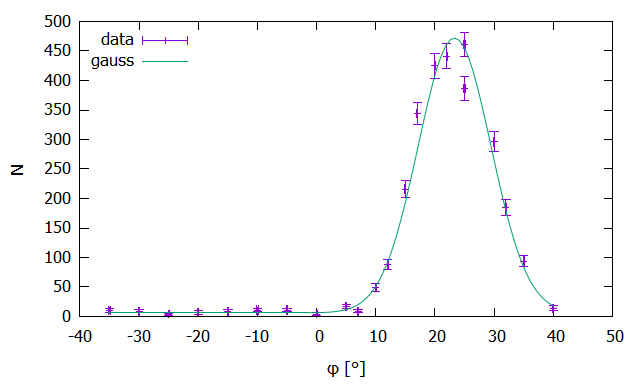
\includegraphics[width=\textwidth]{jeden0.png}
\caption{$\Psi="0\dg"$}
\label{jeden0}
\end{subfigure}\begin{subfigure}{0.5\textwidth}
\centering
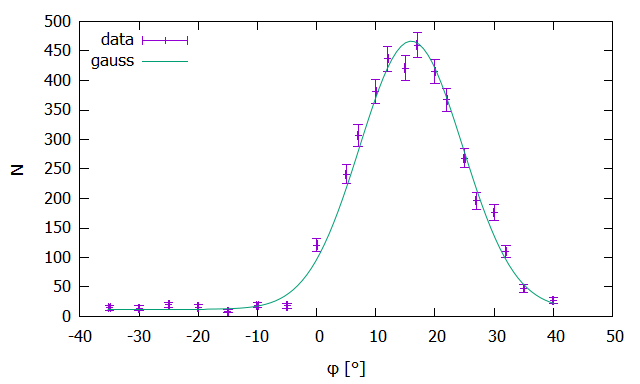
\includegraphics[width=\textwidth]{jeden80.png}
\caption{$\Psi="80\dg"$}
\label{jeden80}
\end{subfigure}
\caption{Úhlové rozdělení koincidencí pro měření s jedním zářičem}
\label{jeden}
\end{figure}
Jelikož počet detekcí v časovém intervalu $t$ je náhodný jev řídící se Poissonovým rozdělením, určíme nejistotu každého bodu jako odmocninu z naměřené hodnoty. %cite poisson
Úhly byly měněny otáčením ramenem s úhlovou stupnicí, ze které bylo možné odečítat úhel na desítky minut, nejistota měření úhlu tedy byla $"5'"\doteq"0,1\dg"$. 
Závislost by teoreticky měla mít podobu funkce vyjadřující plochu překryvu dvou kruhových detektorů v závislosti na úhlu. % výpočet?
Protože jsou však plochy detektorů dostatečně velké, můžeme tuto funkci aproximovat Gaussovou funkcí. Prokládáme tedy naměřenou závislost funkcí
\eq{
N(\Phi)=A*e^{-\frac{(\Phi-B)^2}{C}}+D\,.
}
Fitování jsme prováděli pomocí programu GNUPLOT se zahrnutím jednotlivých nejistot a získané hodnoty uvedli do tabulky \ref{konstanty1}.
\begin{table}[h]
\centering
\caption{Získané fitovací konstanty pro měření s jedním zářičem}
\label{konstanty1}
\begin{tabular}{|c|c|c|c|}
\hline
&$\Psi="0 \dg"$&$\Psi="80 \dg"$\\
\hline
A&	466$\pm$19&454$\pm$	17\\
B&	23,3$\pm$0,2&	16,0$\pm$0,3\\
C&	76$\pm$5&156$\pm$10\\
D&	6$\pm$2&	12$\pm$	3\\
\hline
\end{tabular}
\end{table}
Parametr A zde má význam maximální incidence, parametr B maxima rozložení, parametr C je dvojnásobek rozptylu $C=2\sigma^2$ a parametr D je přirozené pozadí náhodných koincidencí. Rozptyl je pro druhé měření na $\Psi="80 \dg"$ větší, což může být způsobeno větší blízkostí zdroje k jednomu z detektorů, díky které mají detektory zdroj \uv{mezi sebou} pro větší prostorový úhel.

Maximum rozložení se tedy pro úhel $\Psi_1="(0\pm0,1) \dg"$ bylo $\Phi_1="(23,3\pm0,2) \dg"$ a pro úhel $\Psi_2="(80,0\pm0,1) \dg"$ bylo $\Phi_1="(16,0\pm0,3) \dg"$.
Z těch můžeme pomocí vzorců \eqref{primka}, \eqref{mat},  \eqref{mat2},  \eqref{x} a  \eqref{y}.
vypočítat polohu zářiče, pro vzálenost $R="(15,0\pm0,3) cm"$ které byla $x="(2,5\pm0,2) cm"$ a $y="(3,60\pm0,09) cm"$. 
%TODO obrázek?
\subsection*{Jeden zářič velké úhly}
Při měření koincidencí pro velké úhly (při kterých není lebka mezi detektory, tudíž nemůže docházet k pravým koincidencím) jsme pro měření po dobu $"100 s"$ dostali hodnotu $90\pm9$ záchytů pro úhel $\Phi = "90\dg"$ avšak pro úhel $\Phi="150 \dg"$ jsme dostali $277\pm17$ záchytů.  Při zachování úhlu $\Phi="150 \dg"$ a položení plechu mezi detektory byla naměřena hodnota $129\pm11$. U všech měření byla nejistota určena jako odmocnina z naměřené hodnoty, protože počet záchytů má Poissonovské rozdělení. Nejistota měření úhlu je opět $"0,1 \dg"$.
\subsection*{Dva zářiče}
Pro měření se dvěma zářiči byla opět použita doba měření $"20 s"$ a byly měřeny rozsahy úhlů $\Phi$ od $"-35\dg"$ po $"35\dg"$ pro $\Psi="0\dg"$, od $"-45\dg"$ po $"35\dg"$ pro $\Psi="-90\dg"$ a pro poslední měření pro $\Psi="60\dg"$ již byly měřeny pouze okolí předpokládaných peaků. Všechna měření byla prováděna s krokem $"5\dg"$ a nejistota jednotlivých měření byla určena jako odmocnina z naměřené hodnoty koincidencí. Naměřené hodnoty jsou uvedeny v tabulce \ref{dvazarice} jednotlivé závislosti zakresleny v grafech na obrázcích \ref{dva0}, \ref{dva90} a \ref{dva60}.
\begin{table}[h]
\centering
\caption{Naměřené hodnoty koincidencí pro měření se dvěma zářiči}
\label{dvazarice}
\begin{tabular}{|c|c|c|c|c|c|c|}
\hline
&\multicolumn{2}{c|}{$\Psi="0 \dg"$}&\multicolumn{2}{c|}{$\Psi="-90 \dg"$}&\multicolumn{2}{c|}{$\Psi="60 \dg"$}
\\
\hline
\popi{\Phi}{\dg}&$n$&$\sigma(n)$&$n$&$\sigma(n)$&$n$&$\sigma(n)$
\\
\hline
-45&-&-&23&5&-&-
\\
\hline
-40&-&-&67&8&-&-
\\
\hline
-35&23&5&247&16&-&-
\\
\hline
-30&27&5&450&21&-&-
\\
\hline
-25&37&6&631&25&-&-
\\
\hline
-20&80&9&431&21&121&11
\\
\hline
-15&261&16&193&14&255&16
\\
\hline
-10&491&22&42&6&353&19
\\
\hline
-5&580&24&103&10&333&18
\\
\hline
0&523&23&245&16&197&14
\\
\hline
5&378&19&364&19&-&-
\\
\hline
10&276&17&304&17&-&-
\\
\hline
15&174&13&135&12&232&15
\\
\hline
20&68&8&42&6&422&21
\\
\hline
25&29&5&21&5&590&24
\\
\hline
30&25&5&17&4&506&22
\\
\hline
35&24&5&14&4&249&16
\\
\hline
\end{tabular}
\end{table}
\begin{figure}
\centering
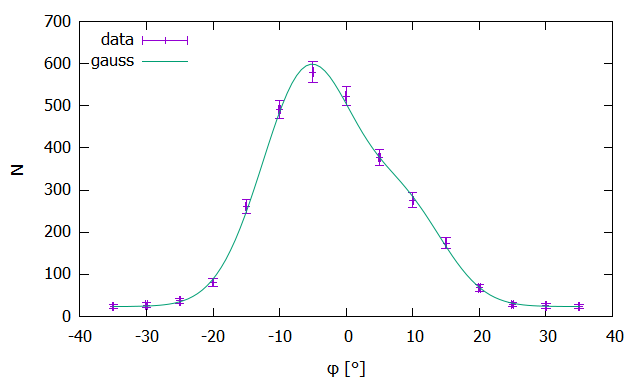
\includegraphics[width=\textwidth]{dva0.png}
\caption{Úhlové rozdělení koincidencí pro měření se dvěma zářiči pro $\Psi="0\dg"$}
\label{dva0}
\end{figure}
\begin{figure}
\centering
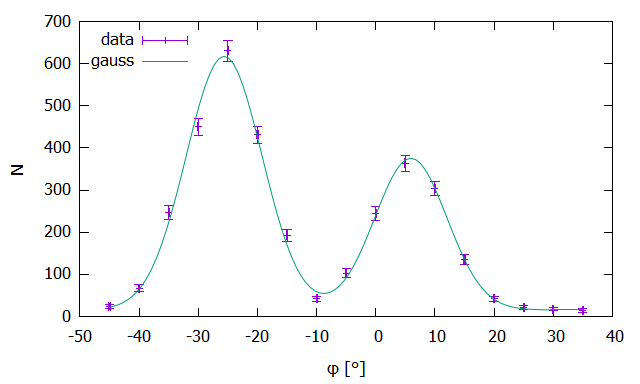
\includegraphics[width=\textwidth]{dva90.png}
\caption{Úhlové rozdělení koincidencí pro měření se dvěma zářiči pro $\Psi="-90\dg"$}
\label{dva90}
\end{figure}
\begin{figure}
\centering
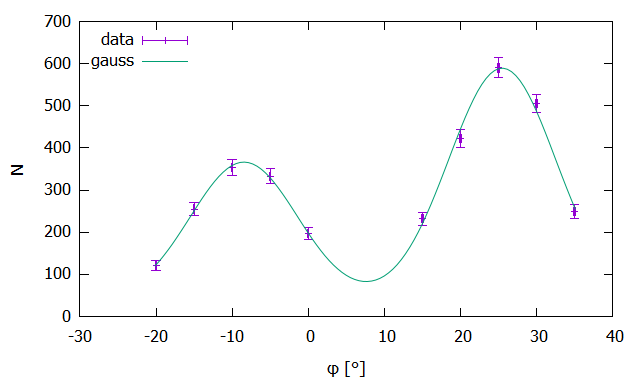
\includegraphics[width=\textwidth]{dva60.png}
\caption{Úhlové rozdělení koincidencí pro měření se dvěma zářiči pro $\Psi="60\dg"$}
\label{dva60}
\end{figure}
Tvar maxim byl opět v přiblížení považován za Gaussovo rozdělení, tudíž byly naměřené hodnoty v programu GNUPLOT fitovány součtem dvou normálních rozdělení ve tvaru
\eq{
N(\Phi)=A*e^{-\frac{(\Phi-B)^2}{C}}+D*e^{-\frac{(\Phi-E)^2}{F}}+G\,.
}
Získané hodnoty parametrů pro jednotlivé grafy jsou uvedeny v tabulce \ref{params2}.
\begin{table}[h]
\centering
\caption{Získané hodnoty fitovacích parametrů pro měření se dvěma zářiči}
\label{params2}
\begin{tabular}{|c|c|c|c|}
\hline
koeficent&$\Psi="0 \dg"$&$\Psi="-90 \dg"$&$\Psi="60 \dg"$
\\
\hline
A&558$\pm$23&602$\pm$24&330$\pm$66
\\
\hline
B&-5,7$\pm$0,6&-25,6$\pm$0,2&-8,4$\pm$0,3
\\
\hline
C&96$\pm$9&82$\pm$5&100$\pm$41
\\
\hline
D&222$\pm$29&360$\pm$20&553$\pm$69
\\
\hline
E&8,9$\pm$1,2&5,9$\pm$0,3&25,6$\pm$0,2
\\
\hline
F&78$\pm$14&75$\pm$7&100$\pm$23
\\
\hline
G&24$\pm$2&16$\pm$3&36$\pm$72
\\
\hline
\end{tabular}
\end{table}
Z parametrů B a E jsme tedy získali polohy maxim, kdy po spárování aktivního zářiče s většími peaky a méně aktivního zářiče s menšími peaky dostaneme s využitím vztahů \eqref{primka}, \eqref{mat},  \eqref{mat2},  \eqref{x} a  \eqref{y}.
polohy obou zářičů X a Y. Ty vypočítáme vždy jako průsečíky každé dvojice přímek, tedy pro každý zářič máme tři polohy. Ty byly v rámci chyby stejné, tudíž můžeme za výsledek považovat jejich aritmetický průměr, tedy:
\eq[m]{
X_1&="[-3,2\pm0,1;0,9\pm0,2] cm"\\
X_2&="[-3,2\pm0,6;0,9\pm2,1] cm"\\
X_3&="[-3,2\pm0,2;0,9\pm0,2] cm"\\
X&="[-3,2\pm0,3;0,9\pm0,2] cm"\\
Y_1&="[0,81\pm0,03;-0,8\pm0,1] cm"\\
Y_2&="[0,8\pm0,1;-0,8\pm0,3] cm"\\
Y_3&="[0,8\pm0,2;-0,8\pm0,1] cm"\\
Y&="[0,8\pm0,1;-0,8\pm0,2] cm"\\
}
\section*{Diskuse}
Úhlové rozdělení počtu koincidencí pro měření s jedním zářičem sice není přímo Gaussova funkce, ale vzorkování je tak málo husté a měření nepřesná, takže s ní můžeme bez problémů rozdělení aproximovat. Zároveň vidíme, že šířka peaku závisí na vzdálenosti zářiče od detektoru A, čím je zářič blíž, tím má peak širší. Měření bychom mohli zpřesnit opakováním měření, hustším vzorkováním nebo delším časem měření.

Pro měření v úhlech, které nemohou odpovídat pravé koincidenci z beta rozpadu se naměřená hodnota zvyšovala. To může být způsobené takzvaným \uv{cross talk}, tedy komunikaci detektorů mezi sebou, kdy fotony comptonovsky rozptýlené na jednom detektoru jsou zachyceny druhým detektorem, což se děje častěji právě kvůli tomu, že se detektory navzájem vidí pod větším prostorovým úhlem. To jsme ověřili tím, že jsme mezi detektory umístili olověný plech, který zachytil rozptýlené fotony a tedy zabránil vzájemné komunikaci detektorů a koincidence se snížila.

Pro měření se dvěma zářiči byly pro první měření zářiče téměř v přímce, tedy jsou oba peaky špatně rozeznatelné a jejich parametry spíše odhadujeme dosazením výchozích parametrů fitu. Všchny tři přímky identifikované ke stejnému zářiči se protínají v rámci chyby v jednom bodě, tedy můžeme polohu zářiče jednoznačně identifikovat, avšak s velkou relativní chybou. Vypočtené polohy zářičů odpovídají polohám získaných graficky pomocí zakreslení do obrázku v rámci praktika i odtajněnému rozložení zářičů v lebce. 
\section*{Závěr}
Měření úhlového rozdělení pro jeden zářič vykazovalo jedno maximum ve tvaru aproximovatelném Gaussovou křivkou, kterou jsme také prokládali. Pro měření s jedním zářičem jsme zjistili jeho polohu jako $"[2,5\pm0,2;3,60\pm0,09] cm"$.
Při měření pro větší úhly $\Phi$ byl pozorován Comptonův rozptyl, což bylo potvrzeno odstíněním jeho efektu vložením olověného plechu mezi detektory.
Pro měření se dvěma zářiči byly naměřena tři úhlová rozložení pro různé úhly $\Psi$ a identifikovány polohy zářičů jako $"[-3,2\pm0,3;0,9\pm0,2] cm"$ a $"[0,8\pm0,1;-0,8\pm0,2] cm"$, což odpovídalo polohám zjištěným graficky.
\section*{Literatura}
\begin{thebibliography}{Per00}
\bibitem{studijnitext}
Studijní text fyzikální praktikum, úloha A7 - Pozitronová emisní tomografie, dostupné z: \url{https://physics.mff.cuni.cz/vyuka/zfp/_media/zadani/texty/txt_407.pdf}, citováno \today
\end{thebibliography}

\end{document}

